\input{../../preamble2.tex}

\begin{document}
\begin{center}
	\Huge\textbf{Математический анализ}
\end{center}
\tableofcontents
\newpage

 \begin{center}
 \large{\textbf{Модуль №1} \\
 \textit{Элементарные функции и пределы}}
 \end{center}
 \input{Основы математического анализа.tex}
 \newpage
 \zerocounter
 \input{Числовая последовательность.tex}
 \newpage
 \zerocounter
 \input{Предел функции.tex}
 \newpage
 \zerocounter
 \input{бмф. Арифметические операции.tex}
 \newpage
 \zerocounter
 \input{Предел функции. бмф ббф.tex}
 \newpage
 \zerocounter
 \input{Непрерывность функции. Точки разрыва.tex}
 \newpage
 \zerocounter
 \begin{center}
 \large{\textbf{Модуль №2} \\
 \textit{Дифференциальное исчисление функции одной переменной}}
 \end{center}
 \input{Производная функции.tex}
 \newpage
 \zerocounter
 \input{Дифференциал функции.tex}
 \zerocounter
%%%%%%%%%%%%%%%%%%%%

\section{Основные теоремы дифференциального исчисления}
\begin{theorem}[\textbf{Теорема Ферма} (о нулях производной)]\hlabel{Ферма}
	Пусть функция $y=f(x)$ определена на промежутке $X$ и во внутренней точке $\bm{c}$ этого промежутка достигает наибольшего или наименьшего значения. Если в этой точке существует производная $f'(c)$, то $f'(c) = 0$.
\end{theorem}
\begin{proof}
	Пусть функция $y=f(x)$ в точке $x=c$ принимает наибольшее значение на промежутке $X\Rightarrow\ \forall x \in X\ \Rightarrow\ f(x)\le f(c)$\\
	Дадим приращение $\Delta x$ в точке $x=c$, тогда $f(c + \Delta x) \le f(c)$.\\[1ex]
	Пусть $\exists\ f'(c) = \lim\limits_{\Delta x \to 0}\dfrac{\Delta y}{\Delta x} = \lim\limits_{\Delta x \to 0}\dfrac{y(c+ \Delta x) - y(c)}{\Delta x}$\\[1ex]
	Рассмотрим два случая:
	\begin{enumerate}
		\item $\Delta x > 0,\ \Delta x \to 0+,\ x \to c+$
		      \begin{flalign*}
			       & f'_+(c) = \lim_{\Delta x \to 0+}\frac{y(c+ \Delta  x) - y(c)}{\Delta x} = \left( \frac{-}{+}\right) \le 0 &
		      \end{flalign*}
		\item $\Delta x < 0,\ \Delta x \to 0-,\ x \to c-$
		      \begin{flalign*}
			       & f'_-(c) = \lim_{\Delta x \to 0-}\frac{y(c+ \Delta  x) - y(c)}{\Delta x} = \left( \frac{-}{-}\right) \ge 0 &
		      \end{flalign*}
	\end{enumerate}
	По теореме \textit{о существовании производной функции в точке} (\textbf{С.\pageref{Существование производной функции в точке}, Т. \ref{Существование производной функции в точке}}):
	\begin{gather*}
		f'(c) = f'_+(c) = f'_-(c) = 0
	\end{gather*}
\end{proof}
\subsubsection*{Геометрический смысл теоремы Ферма}
\begin{minipage}{15cm}
	\begin{wrapfigure}[4]{r}{0.35\textwidth}
		\vspace{-2\topsep}
		\begin{tikzpicture}[very thick, scale=0.7]
			\tkzInit[xmin=-1, xmax=8, ymin=-1, ymax=5]
			%	\tkzGrid
			\tkzDrawX[thick] \tkzDrawY[thick]
			\node[below left] at (0, 0) {$0$};
			\draw (2, 1) .. controls (3.2, 4.5) and (4.8, 4.5) .. (6, 2) node[right]{$y=f(x)$};
			\draw (1, 3.77) -- (8.5, 3.77) node[above]{\footnotesize{касательная}};
			\draw[dotted] (4.2, 0) node[below]{$c$} -- (4.2, 3.77) node[above]{\footnotesize{наибольшее}};
			\node[left] at (0, 3.77) {$f(c)$};
		\end{tikzpicture}
	\end{wrapfigure}
	Касательная к графику функции $y=f(x)$ \\
	в точке $(c, f(c))$ параллельна оси абсцисс.\\
	$f(c)$ -- наибольшее значение функции
\end{minipage}\vspace{10\topsep}
\begin{theorem}[\textbf{Теорема Ролля}]\hlabel{Ролль}
	Пусть $y=f(x)$
	\begin{enumerate}
		\item непрерывна на $[a;b]$
		\item дифференцируема на $(a;b)$
		\item $f(a) = f(b)$
	\end{enumerate}
	Тогда $\exists\ c \in (a;b)\colon f'(c) = 0$
\end{theorem}
\begin{proof}
	Так как функция $y=f(x)$ непрерывна на $[a;b]$, то по теореме \textit{Вейерштрасса} (\textbf{С.\pageref{Вейерштрасса 2}, Т.\ref{Вейерштрасса 2}}) она достигает на этом отрезке своего наибольшего и наименьшего значений.\\
	Возможны два случая:
	\begin{enumerate}
		\item Наибольшее и наименьшее значения достигаются на границе, то есть в точке $a$ и в точке $b$\\
		      $M=m$, где $\begin{aligned}
				       & m \text{ -- наименьшее} \\
				       & M \text{ -- наибольшее}
			      \end{aligned}\ \Rightarrow\ y=f(x)=const \text{ на } [a;b]\ \Rightarrow\\[1ex]
			      \Rightarrow\ \forall x \in (a;b)\colon f'(x)=0$
		\item Наибольшее или наименьшее значение достигается во внутренней точке $(a;b)$.\\
		      Тогда для функции $y=f(x)$ справедлива теорема \textit{Ферма} (\textbf{Т.\ref{Ферма}}) $\Rightarrow$\\
		      $\Rightarrow\ \exists\ c \in (a;b)\colon f'(c) = 0$
	\end{enumerate}
\end{proof}
\begin{corollary}
	Если $f(a) = f(b) = 0$, то между двумя нулями функции существует хотя бы один нуль производной.
\end{corollary}
\newpage
\begin{theorem}[\textbf{Теорема Лагранжа}]
	Пусть функция $y=f(x)$
	\begin{enumerate}
		\item непрерывна на $[a;b]$
		\item дифференцируема на $(a;b)$
	\end{enumerate}
	Тогда $\exists\ c \in (a;b)\colon \boxed{f(b) - f(a) = f'(c) \cdot (b-a)}$
\end{theorem}
\begin{proof}
	Рассмотрим вспомогательную функцию: $F(x) = f(x) - f(a) - \dfrac{f(b) - f(a)}{b - a} \cdot (x-a)$\\
	$F(x)$ непрерывна на $[a;b]$ как сумма непрерывных функций.\\
	Существует конечная производная функции $F(x)$. \vspace{-\topsep}
	\begin{flalign*}
		 & F'(x) = f'(x) - \frac{f(b) - f(a)}{b-a} \Rightarrow\ \begin{aligned}  & \text{по необходимому и достаточному} \\
                 & \text{условию дифференцируемости }\end{aligned}\ (\textbf{С.\pageref{Условие дифференцируемости}, Т.\ref{Условие дифференцируемости}}) \Rightarrow & \\
		 & \Rightarrow\ F(x) \text{ -- дифференцируема на } (a;b)                                                                                                &
	\end{flalign*}
	Покажем, что $F(a) = F(b)$:
	\begin{flalign*}
		 & F(a) = f(a) - f(a) - \frac{f(b) - f(a)}{b - a} \cdot(a - a) = 0                             & \\
		 & F(b) = f(b) - f(a) - \frac{f(b) - f(a)}{b - a} \cdot(b - a) = f(b) - f(a) - f(b) + f(a) = 0 &
	\end{flalign*}
	$\Rightarrow\ F(x)$ удовлетворяет условиям теоремы \textit{Ролля} (\textbf{Т. \ref{Ролль}}) \\
	По теореме \textit{Ролля} $\Rightarrow\ \exists\ c \in (a;b) \qquad F'(c) = 0$
	\begin{flalign*}
		 & F'(x) = f'(x) - \frac{f(b) - f(a)}{b - a}     & \\
		 & F'(c) = f'(c) - \frac{f(b) - f(a)}{b - a} = 0 & \\
		 & f'(c) = \frac{f(b) - f(a)}{b - a}             & \\
		 & f(b) - f(a) = f'(c) \cdot (b-a)
	\end{flalign*}
\end{proof}
\subsubsection*{Геометрический смысл теоремы Лагранжа}
\begin{figure}[h]
	\centering
	\begin{tikzpicture}[very thick, scale=0.8, font=\footnotesize]
		\tkzInit[xmin=-1, xmax=8, ymin=-1, ymax=5]
		%	\tkzGrid
		\tkzDrawX[thick] \tkzDrawY[thick]
		\node[below left] at (0, 0) {$0$};
		\tkzDefPoint(1.5, 1.5){A}
		\tkzDefPoint(5, 1.5){C}
		\tkzDefPoint(5, 3.5){B}
		\tkzDefPoint(0.5, 1.5){k1}
		\tkzDefPoint(4.8, 4.15){k2}

		\draw (A) -- (B);
		\draw (A) to [out=60, in=183] (B);
		\draw (k1) -- (k2) node[midway, above left, rotate=31.5]{\scriptsize{касательная}};
		\draw[dotted] (0, 1.5) node[left]{$f(a)$} -- (C) node[right]{$C$};
		\draw[dotted] (0, 3.5) node[left]{$f(b)$} -- (B) node[above]{$B$} node[right=5pt]{$y=f(x)$};
		\draw[dotted] (A) node[below left]{$A$} -- (1.5, 0) node[below]{$a$};
		\draw[dotted] (B) -- (5, 0) node[below]{$b$};
		\draw[dotted] (2.8, 0) node[below]{$c$} -- (2.8, 2.9);

		\tkzDrawPoint[size = 2pt](A)
		\tkzDrawPoint[size = 2pt](C)
		\tkzDrawPoint[size = 2pt](B)
		\tkzMarkAngle[mark=none, thin, size=0.8](C,A,B)
		\tkzLabelAngle[pos=1.1, font=\footnotesize](C,A,B){$\alpha$}
		\tkzMarkAngle[mark=none, thin, size=0.5](C,k1,k2)
		\tkzLabelAngle[pos=0.75, font=\scriptsize](C,k1,k2){$\alpha'$}

		\node at (9.5, 5) {$A\big(a, f(a)\big)$};
		\node at (9.5, 4.3) {$B\big(b, f(b)\big)$};
		\node at (9.65, 3.4) {$\tg \alpha = \dfrac{BC}{AC}$};
		\node at (9.7, 2.5) {$\tg \alpha' = \tg \alpha$};

	\end{tikzpicture}
\end{figure}
\newpage
\begin{theorem}[\textbf{Теорема Коши}]\label{Коши}
	Пусть функции $f(x)$ и $\varphi (x)$
	\begin{enumerate}
		\item непрерывны на $[a;b]$
		\item дифференцируемы на $(a;b)$
		\item $\forall x \in (a;b)\colon \varphi' (x) \ne 0$
	\end{enumerate}
	Тогда $\exists\ c \in (a;b)\colon$ \vspace{-\topsep}
	\begin{gather*}
		\boxed{\frac{f(b) - f(a)}{\varphi (b) - \varphi (a)} = \frac{f'(c)}{\varphi'(c)}}
	\end{gather*}
\end{theorem} 
\begin{proof}
	Рассмотрим вспомогательную функцию:
	\begin{gather*}
		F(x) = f(x) - f(a) - \frac{f(b) - f(a)}{\varphi(b) - \varphi(a)} \cdot \Big(\varphi(x) - \varphi(a)\Big)
	\end{gather*}
	\begin{enumerate}
		\item $F(x)$ непрерывна на $[a;b]$ как линейная комбинация непрерывных функций
		\item $F(x)$ дифференцируема на $(a;b)$ как линейная комбинация дифференцируемых функций
		\item $F(a) = F(b)$
	\end{enumerate}\vspace{-\topsep}
	\begin{flalign*}
		 & F(a) = \cancel{f(a)} - \cancel{f(a)} - \frac{f(b)-f(a)}{\varphi(b) - \varphi(a)}\cdot(\underbrace{\varphi(a) - \varphi(a)}_{0})=0                             & \\
		 & F(b) = f(b) - f(a) - \frac{f(b) - f(a)}{\cancel{\varphi(b) - \varphi(a)}}\cdot\Big(\cancel{\varphi(b)-\varphi(a)}\Big)= \cancel{f(b)}- \bcancel{f(a)} - \cancel{f(b)} + \bcancel{f(a)} = 0 &
	\end{flalign*}
	Функция $F(x)$ удовлетворяет условию теоремы \textit{Ролля} (\textbf{Т.\ref{Ролль}}).\\
	По теореме \textit{Ролля} $\Rightarrow$ $\exists\ c \in (a;b)\colon F'(c) = 0$\\[1ex]
	Вычислим $F'(x) = f'(x) -\dfrac{f(b)-f(a)}{\varphi(b) - \varphi(a)}\cdot \varphi'(x)$
	\begin{flalign*}
		 & F'(c) = f'(c) - \frac{f(b) - f(a)}{\varphi(b) - \varphi(a)} \cdot \varphi'(c) = 0 & \\
		 & \frac{f(b)-f(a)}{\varphi(b) - \varphi(a)}\cdot \varphi'(c) = f'(c)                & \\
		 & \frac{f(b) - f(a)}{\varphi(b) - \varphi(a)}=\frac{f'(c)}{\varphi'(c)}
	\end{flalign*}
\end{proof}
\newpage
\zerocounter
\subsection{Правило Лопиталя-Бернулли}
\begin{theorem}
	Пусть $f(x)$ и $\varphi(x)$:
	\begin{enumerate}
		\item определены и дифференцируемы в $\mathring{S}(x_0)$
		\item $\lim\limits_{x \to x_0}f(x) = 0$;\quad $\lim\limits_{x\to x_0}\varphi(x) = 0$
		\item $\forall x \in \mathring{S}(x_0)\colon \varphi'(x)\ne 0$
		\item $\exists \lim\limits_{x \to x_0}\dfrac{f'(x)}{\varphi'(x)}= A$,\quad $A$ --- конечное или $\infty$
	\end{enumerate}
	Тогда $\exists \lim\limits_{x \to x_0} \dfrac{f(x)}{\varphi(x)} = \lim\limits_{x \to x_0}\dfrac{f'(x)}{\varphi'(x)}=A$
\end{theorem}
\begin{proof}
	Доопределим функции $f(x)$ и $\varphi(x)$ в точке $x_0$ нулём.\\
	Пусть $\left\{\begin{aligned}
			f(x_0) = 0 \\
			\varphi(x_0)=0
		\end{aligned}\right.$\\
	\begin{flalign*}
		 & \text{По условию 2) } \Rightarrow\ \left. 
			\begin{aligned}
				& \lim_{x \to x_0} f(x) = 0 = f(x_0) \\
				& \lim_{x \to x_0} \varphi(x) = 0 = \varphi(x)
			\end{aligned} \right\}\ \Rightarrow\ \begin{aligned}
				&\text{по определению непрерывной}\\
				&\text{функции в точке, } f(x) \text{ и } \varphi(x) \\
				&\text{непрерывны в точке }x_0. \end{aligned} &
	\end{flalign*}
	По условию 1) функции  $f(x)$ и $\varphi(x)$ дифференцируемы в $\mathring{S}(x_0) \Rightarrow$ по теореме \textit{о связи дифференцируемости и непрерывности} (\textbf{С.\pageref{Связь диф. и непр. функции}, Т. \ref{Связь диф. и непр. функции}}) $\Rightarrow f(x)$ и $\varphi(x)$ непрерывны в $\mathring{S}(x_0)$.\\
	Таким образом, $f(x)$ и $\varphi(x)$ непрерывны в $S(x_0)$.
	\begin{center}
	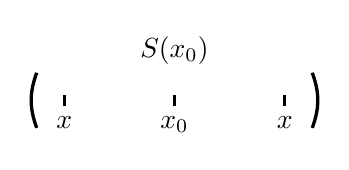
\begin{tikzpicture}[very thick,scale=0.7]
		\tkzInit[xmin=-4, xmax=4, ymin=0, ymax=0]
		\tkzDrawX[thick]
		% \tkzGrid
		\draw (0, -0.1) node[below]{$x_0$}-- (0, 0.1) node[above=7pt]{$\large{S(x_0)}$};
		\draw (-2, -0.1) node[below]{$x$}-- (-2, 0.1);
		\draw (2, -0.1) node[below]{$x$}-- (2, 0.1);
		\draw (-2.5,0.5) to [out=-110, in=110] (-2.5, -0.5);
		\draw (2.5,0.5) to [out=-70, in=70] (2.5, -0.5);
	\end{tikzpicture}\qquad $ \forall x \in S(x_0) \qquad [x_0; x] \text{ или } [x; x_0] $
	\end{center}
	функции $f(x)$ или $\varphi(x)$ удовлетворяют условию теоремы \textit{Коши} (\textbf{Т.\ref{Коши}}) на $[x_0; x]$.\\
	По теореме \textit{Коши} $\exists\ c \in (x_0; x)\colon$
	\begin{gather*}
		\frac{f(x) - f(x_0)}{\varphi(x)-\varphi(x_0)}=\frac{f'(c)}{\varphi'(c)} \tag{$*$}
	\end{gather*}
	\begin{flalign*}
	& \text{Так как } f(x_0) = 0,\ f(x_0) = 0\ \Rightarrow\ \boxed{\displaystyle\frac{f(x)}{\varphi(x)} = \displaystyle\frac{f'(c)}{\varphi'(c)}} \tag{$*$} &\\
	& \text{Так как } \exists \lim\limits_{x \to x_0} \frac{f'(x)}{\varphi'(x)} = A\colon &
	\end{flalign*}
	\begin{minipage}{16cm}
	\begin{wrapfigure}[2]{r}{0.4\textwidth}
		\vspace{-4\topsep}
		\begin{tikzpicture}[very thick,scale=0.7, >=stealth]
			\tkzInit[xmin=-2, xmax=2, ymin=-1, ymax=1]
			% \tkzGrid
			\draw[<->] (-2,0) -- (2,0);
			\draw (-2, -0.2) node[below]{$x_0$}-- (-2, 0.2);
			\draw (2, -0.2) node[below]{$x$}-- (2, 0.2);
			\draw (0, -0.1) node[above]{$c$}-- (0, 0.1);
			\draw[->] (2, -1) to [out=190, in=350] (-2, -1);
			\node at (4, 0) {$\footnotesize{\begin{aligned} &x \to x_0 \\ & c \to x_0 \end{aligned}}$};
		\end{tikzpicture}
	\end{wrapfigure}
	Правая часть $(*)\colon \lim\limits_{c \to x_0} \dfrac{f'(c)}{\varphi'(c)} \xlongequal{\text{4)}} A $
	\end{minipage}\\[1ex] 
	Левая часть $(*)\colon \lim\limits_{x \to x_0} \dfrac{f(x)}{\varphi(x)} = \lim\limits_{c \to x_0}\dfrac{f'(c)}{\varphi'(c)}=A$\\[1ex]
	Получаем, что $\lim\limits_{x\to x_0}\dfrac{f(x)}{\varphi(x)}=\lim\limits_{x \to x_0}\dfrac{f'(x)}{\varphi'(x)} = A$
\end{proof}
\begin{theorem}
	Пусть функции $f(x)$ и $\varphi(x)$:
	\begin{enumerate}
		\item определены и дифференцируемы в $S(x_0)$
		\item $\lim\limits_{x \to x_0}f(x) = \infty,\quad \lim\limits_{x \to x_0} \varphi(x) = \infty $
		\item $\forall x \in \mathring{S}(x_0)\colon \varphi'(x) \ne 0$
		\item $\exists \lim\limits_{x \to x_0} \dfrac{f'(x)}{\varphi'(x)} = A $
	\end{enumerate}
	Тогда $\exists \lim\limits_{x \to x_0} \dfrac{f(x)}{\varphi(x)} = \lim\limits_{x \to x_0} \dfrac{f'(x)}{\varphi'(x)} = A $
\end{theorem}
\subsection{Сравнение показательной, степенной и логарифмической функции на бесконечности}
Пусть\quad $\begin{aligned}
		 & f(x) = x^{n},\ n \in \N         \\
		 & g(x) = a^x,\ a>1                \\
		 & h(x) = \ln x\qquad 
	\end{aligned}\qquad x\to +\infty $
\begin{flalign*}
	 & \lim_{x\to +\infty} \frac{f(x)}{g(x)} = \lim_{x\to +\infty} \frac{x^n}{a^x} = \left(\frac{\infty}{\infty}\right) \xlongequal{\text{Л-Б}} \lim_{x\to +\infty}\frac{n\cdot x^{n-1}}{a^x\cdot \ln a} = \left(\frac{\infty}{\infty}\right) \xlongequal{\text{Л-Б}} &\\
	 & \xlongequal{\text{Л-Б}} \underset{n \text{ раз }}{\text{\ldots}} \xlongequal{\text{Л-Б}} \lim_{x\to +\infty}\frac{n\cdot (n-1)\cdot(n-2)\cdot\ldots\cdot 1}{a^x(\ln a)^n}= \frac{n!}{\ln^n a}\cdot \lim_{x\to +\infty}\frac{1}{a^x}=\frac{n!}{\ln^n a}\cdot 0 = 0&
\end{flalign*}
$a^x$ растёт быстрее, чем $x^n$ при $x\to +\infty$ или $x^n = o(a^x)$ при $x\to +\infty$
\begin{flalign*}
	 & \lim_{x\to +\infty}\frac{h(x)}{f(x)}=\lim_{x\to +\infty}\frac{\ln x}{x^n}=\left(\frac{\infty}{\infty}\right) = \lim_{x\to +\infty}\frac{\frac{1}{x}}{n\cdot x^{n-1}} = \frac{1}{n}\cdot \lim_{x\to +\infty} \frac{1}{x^n}=\frac{1}{n}\cdot 0 = 0 &
\end{flalign*}
$x^n$ растёт быстрее, чем $\ln x$ при $x\to +\infty$ или $\ln x = o(x^n)$ при $x\to +\infty$\\[1ex]
$\left. \begin{array}{lclll}
	\text{Вывод:} & 1. & g(x) = a^x & , & a>1\\
	& 2. & f(x) = x^n & , & n\in \N\\
	& 3. & h(x) = \ln x & & 
\end{array} \right\uparrow\quad x\to +\infty$
\zerocounter
\newpage
\subsection{Формула Тейлора. Многочлены Тейлора}
\begin{theorem}
	Пусть функция $y=f(x)$ $n$ раз дифференцируема в точке $x_0$ и определена в некоторой окрестности этой точки. Тогда $\forall x \in S(x_0)$ имеет место формула Тейлора:
	\begin{align}
		\begin{aligned}
			f(x) =& f(x_0)  + \frac{f'(x_0)}{1!}\cdot (x-x_0) + \frac{f''(x_0)}{2!}\cdot (x-x_0)^2 + \frac{f'''(x_0)}{3!}\cdot (x-x_0)^3 + \\
			              & + \ldots + \frac{f^{(n)}(x_0)}{n!}\cdot (x-x_0)^n + R_n(x)
		\end{aligned}
	\end{align}
	Кратко: $f(x) = P_n(x) + R_n(x)$, где
	\begin{flalign*}
		&\begin{aligned}
		P_n(x) =& f(x_0)  + \frac{f'(x_0)}{1!}\cdot (x-x_0) + \frac{f''(x_0)}{2!}\cdot (x-x_0)^2 + \frac{f'''(x_0)}{3!}\cdot (x-x_0)^3 + \\
		& + \ldots + \frac{f^{(n)}(x_0)}{n!}\cdot (x-x_0)^n \hspace{2cm} \text{--- многочлен Тейлора}\qquad x\to x_0
		\end{aligned}  &
	\end{flalign*}
	$R_n(x)$ --- остаточный член формулы Тейлора
\end{theorem}
\begin{proof}
	Покажем, что такой многочлен существует. Будем искать многочлен Тейлора в виде:
	\begin{gather}
		P_n(x) = a_0 + a_1(x-x_0) + a_2(x-x_0)^2 + a_3(x-x_0)^3 + a_4(x-x_0)^4 + \ldots + a_n(x-x_0)^n
	\end{gather}
	$a_1, a_2, \ldots, a_n \text{ --- } const$\\ \vspace{-2\topsep}
	\begin{flalign}
		&\text{Пусть выполнено условие: } \left\{\begin{aligned}
			        & P_n(x_0) = f(x_0)                     \\
			        & P'_n(x_0) = f'(x_0)                   \\
			        & P''_n(x_0) = f''(x_0)                 \\
			        & \ldots\ldots\ldots\ldots\ldots\ldots  \\
			        & P^{(n)}_n(x_0) = f^{(n)}(x_0)
		       \end{aligned}\right.&
	\end{flalign}
	$f'(x_0), f''(x_0), \ldots, f^{(n)}(x_0)$ -- существуют, так как $y=f(x)$ $n$ раз дифференцируема в точке $x_0$.\\
	Вычислим $P'_n(x),\ldots,P_n^{(n)}(x)$:
	\begin{flalign*}
		 & P_n(x) = a_0 + a_1(x-x_0) + a_2(x-x_0)^2 + a_3(x-x_0)^3 + a_4(x-x_0)^4 + \ldots + a_n(x-x_0)^n                                                & \\
		 & P'_n(x) = a_1\cdot 1 + a_2\cdot 2(x-x_0) + a_3\cdot 3(x-x_0)^2 + a_4\cdot 4(x-x_0)^3 + \ldots + a_n\cdot n(x-x_0)^{n-1}\hspace*{-7pt}              & \\
		 & P''_n(x) = a_2\cdot 2\cdot 1 + a_3\cdot 3\cdot 2(x-x_0) + a_4\cdot 4\cdot 3(x-x_0)^2 + \ldots + a_n\cdot n\cdot (n-1)(x-x_0)^{n-2}\hspace*{-7pt} & \\
		 & P''_n(x) = a_3\cdot 3\cdot 2\cdot 1 + a_4\cdot 4\cdot 3\cdot 2(x-x_0) + \ldots + a_n\cdot n\cdot (n-1)\cdot (n-2)(x-x_0)^{n-3}              & \\
		 & \ldots \ldots \ldots\ldots\ldots\ldots\ldots\ldots\ldots\ldots\ldots\ldots\ldots\ldots\ldots\ldots\ldots\ldots\ldots\ldots\ldots\ldots\ldots\ldots\ldots\ldots\ldots\ldots                                                                                                                    & \\
		 & P_n^{(n)}(x) = a_n\cdot n(n-1) \cdot (n-2) \cdot\ldots\cdot 1 = a_n \cdot n!
	\end{flalign*} \
	$ x = x_0$
	\begin{flalign*}
		&\left\{\begin{aligned}
			        & P_n(x_0) = a_0                             \\
			        & P'_n(x_0) = 1\cdot a_1                     \\
			        & P''_n(x_0) = 1\cdot 2 \cdot a_2            \\
			        & P'''_n(x_0) = 1\cdot 2 \cdot 3 \cdot a_3   \\
			        & \ldots\ldots\ldots\ldots\ldots\ldots\ldots \\
			        & P^{(n)}_n(x_0) = n!\cdot a_n
		       \end{aligned} \right.\ \overset{(3)}{\Longrightarrow} \left\{
				\begin{aligned}
					& P_n(x_0) = a_0 = f(x_0)                                      \\
					& P'_n(x_0) = 1\cdot a_1 = f'(x_0)                             \\
					& P''_n(x_0) = 1\cdot 2 \cdot a_2 = f''(x_0)                   \\
					& P'''_n(x_0) = 1\cdot 2 \cdot 3 \cdot a_3 = f'''(x_0)         \\
					& \ldots\ldots\ldots\ldots\ldots\ldots\ldots\ldots\ldots\ldots \\
					& P^{(n)}_n(x_0) = n!\cdot a_n = f^{(n)}(x_0)
		        \end{aligned} \right. &
	\end{flalign*}
	\begin{flalign*}
		& \text{Выразим } a_0, a_1, \ldots, a_n\colon \left\{
			\begin{aligned}
		 & a_0 = f(x_0)                  \\
		 & a_1 = \frac{f'(x_0)}{1!}      \\
		 & a_2 = \frac{f''(x_0)}{2!}     \\
		 & a_3 = \frac{f'''(x_0)}{3!}    \\
		 & \ldots\ldots\ldots\ldots      \\
		 & a_n = \frac{f^{(n)}(x_0)}{n!} \\
			\end{aligned}
		\right. &
	\end{flalign*}
	Подставим $a_0, a_1, \ldots, a_n$ в (2):
	\begin{flalign*}
		&\begin{aligned}
		 P_n(x) = f(x_0) &+ \frac{f'(x_0)}{1!}\cdot (x-x_0) + \frac{f''(x_0)}{2!} \cdot(x-x_0)^2 + &\\
		& + \frac{f'''(x_0)}{3!} \cdot (x-x_0)^3 + \ldots + \frac{f^{(n)}(x_0)}{n!} \cdot (x-x_0)^n &
		\end{aligned} \text{ -- многочлен Тейлора}&
	\end{flalign*}
\end{proof}
\begin{theorem}
	Пусть функция $y=f(x)$ $n$ раз дифференцируема в точке $x_0$, тогда
	\begin{gather*}
		x\to x_0\qquad \boxed{R_n (x) = o\big((x-x_0)^n\big)} \text{ --- форма Пеано.}
	\end{gather*}
\end{theorem}
\begin{proof}
	Формула Тейлора: \vspace{-\topsep}
	\begin{flalign*}
		 & f(x) = P_n(x) + R_n(x) & \\
		 & R_n(x) = f(x) - P_n(x) &
	\end{flalign*}
	В силу условия (3):
	\begin{align*}
		 & R_n(x_0) = f(x_0) - P_n(x_0) \xlongequal{\text{(3)}} f(x_0) - f(x_0) = 0 \\
		 & R_n'(x_0) = f'(x_0) - P'_n(x_0) \xlongequal{\text{(3)}} f'(x_0) - f'(x_0) = 0 \\
		 & \ldots \ldots \ldots \ldots\ldots\ldots\ldots\ldots\ldots\ldots\ldots\ldots\ldots\ldots\ldots\ldots\ldots\ldots \\
		 & R_n^{(n)}(x_0) = f^{(n)}(x_0) - P^{(n)}_n(x_0) \xlongequal{\text{(3)}} f^{(n)}(x_0) - f^{(n)}(x_0) = 0
	\end{align*}
	Вычислим:
	\begin{flalign*}
		\lim_{x\to x_0}\frac{R_n(x)}{(x-x_0)^n} &= \left(\frac{0}{0}\right) \xlongequal{\text{Л-Б}} \lim_{x\to x_0}\frac{R_n'(x)}{n\cdot(x-x_0)^{n-1}} = \left(\frac{0}{0}\right) \xlongequal{\text{Л-Б}}\ldots =&\\
		& = \lim\limits_{x \to x_0} \frac{R_n^{(n)}(x)}{n\cdot(n-1)\cdot\ldots\cdot 1}= \frac{1}{n'}\cdot R_n^{(n)}(x_0) = \frac{1}{n'} \cdot 0 = 0 &
	\end{flalign*}
	Вывод: $R_n(x) = o\big((x-x_0)^n\big)$ при $x \to x_0$
\end{proof}

%%%%%%%%%%%%%%%%%%%%
\end{document}